
\documentclass[11pt]{article}
\usepackage[margin=1in]{geometry}
\usepackage{amsmath,amssymb,amsthm}
\usepackage{graphicx}
\usepackage{tikz}
\usepackage{hyperref}
\usepackage[backend=biber,style=numeric,sorting=none]{biblatex}
\addbibresource{references.bib}
\usepackage{bm}
% Default physical mapping for dimensionless tau
\newcommand{\taudef}{100\,\mathrm{ps}} % default physical scale
\newcommand{\taudefns}{0.1\,\mathrm{ns}} % same in ns

\usepackage{enumitem}

\title{\textbf{J.U.M.P. --- Joined-Universe Metric Portal}\\
{\large Unified Theory, Equations, and Numerical Studies}}
\author{White Paper}
\date{v11 --- GitHub Release}

\newtheorem{prop}{Proposition}

\begin{document}\maketitle
\begin{abstract}
We present the J.U.M.P. framework with unique equation set (B*, W*, J*, I*, P*, R*, E*, C*, M*, S*) for a transient, causality-preserving spacetime jump via a zero-expansion warp bubble stitched to a traversable throat using QI-admissible negative-energy pulses. We include parameter baselines, numerical demonstrations, an SI-scale case study, and parameter sweeps with minimal amplitudes.
\end{abstract}

See e.g.~\cite{Alcubierre1994,Natario2002,MorrisThorne1988,GaoJafferisWall2017,FordRoman1995} for background.

\section{Unique Equations (Core)}
\paragraph{Default physical time scale.} In this paper we adopt a fixed mapping for the dimensionless pulse width $\tau$: $\tau_{\rm phys}=\tau\,\tau_0$ with $\tau_0=\taudef\ (= \taudefns).$ All reported physical pulse widths use this default unless explicitly stated.

\textbf{Bubble (B1--B3):}
$ds_B^2 = -dt^2 + (dr - v(t)\Phi(r)dt)^2 + r^2 d\Omega^2$ with $(1/r^2)\partial_r(r^2\Phi)=0$ (regularized bump), compact support.
\medskip

\noindent\textbf{Exit (W1--W3):}
$ds_W^2 = -e^{2\Psi} dt^2 + dr^2/(1-b/r) + r^2 d\Omega^2$, throat $b(r_0)=r_0$, $b'(r_0)<1$, gated $b(r;t)=b_0(r)+\alpha(t)\delta b(r)$.
\medskip

\noindent\textbf{Junction (I1--I5):}
$S_{ij}=-\tfrac{1}{8\pi}([K_{ij}]-h_{ij}[K])$, $\sigma(a)= -(4\pi a)^{-1}(\sqrt{U_+}-\sqrt{U_-})$, shell potential $V(a)$, stability by $V''(a_0)>0$.
\medskip

\noindent\textbf{Pulse Law (P1--P4):}
Balanced tri-lobe $T_{kk}$ (ANEC-neutrality $B\ge A/(2\ell)$, QI-bound $A \le C_1/\tau^4 + C_2(\ell,\Delta/\tau)B/\tau$).
\medskip

\noindent\textbf{Raychaudhuri (R1--R4):}
$\Delta\theta \gtrsim 8\pi I_-$ for short negative pulse $I_-=-\int T_{kk}d\lambda$.
\medskip

\noindent\textbf{Matching (M1--M2)} and \textbf{Stability (S1)} as ορισμένα στο κύριο κείμενο.

\section{Baseline Parameter Ranges}
\begin{center}\begin{tabular}{l|c|c}
\hline
Parameter & Symbol & Range \\ \hline
Pulse width & $\tau$ & $10^{-3}$ to $5.0$ (dimensionless demo) \\
Lobe spread & $\ell$ & $[1.1,\,6.0]$ \\
Timing ratio & $\Delta/\tau$ & $[1.2,\,3.0]$ \\
QI constant & $C_1$ & $10^{-3}$ \\
Geom.\ threshold & $I_{\min}$ & $10^{-3}$ \\ \hline
\end{tabular}\end{center}

\section{Numerical Demonstration (Feasible Pulse Example)}
Closed-form Gaussian integrals define $C_2(\ell,\Delta/\tau)$ and yield admissible $(A,\tau,B,\ell,\Delta)$ satisfying ANEC-neutrality and QI.

\section{Numerical Case Study (SI Units)}
We embed an SI-scale example (bubble $R_B=20$ m, shell $0.5$ m, throat $r_0=2$ m, $L_{\rm th}=10$ m, pulse $100$ ps) and plot energy/pressure versus $B$ and $R_B$. See figures in the Case Study section.

\section{Parameter Sweep and Optimization}
\subsection*{Best Pulse Point (from scanned grids)}
\paragraph{Physical scaling of $\tau$ (multi-scale).}\emph{Default mapping:} $\tau_0=\taudef$ ($=\taudefns$).
We report the physical pulse width $\tau_{\rm phys}=\tau\,\tau_0$ for three practical reference scales:
\begin{center}
\begin{tabular}{l|c|c|c}
\hline
Quantity & $\tau_0=1$ ns & $\tau_0=2$ ns & $\tau_0=0.1$ ns \\ \hline
$\tau_{\rm phys}$ & 1.59064 ns & 3.18128 ns & 0.159064 ns \\ \hline
\end{tabular}
\end{center}

\paragraph{Alternative units and control metrics.}
Let the dimensionless $\tau$ map to a physical width via $\tau_{\rm phys}=\tau\,\tau_0$ with default scale $\tau_0=1\,\mathrm{ns}$. For the best point, this gives
\begin{center}
\begin{tabular}{l|c}
\hline
Quantity & Value \\ \hline
$\tau_{\rm phys}$ (for $\tau_0\!=\!1$ ns) & 1.59 ns \\
$20\log_{10}(A^\star)$ [dB] & -72.013 \\
$20\log_{10}(B^\star)$ [dB] & -78.862 \\ \hline
\end{tabular}
\end{center}

These dB values are reported on a dimensionless magnitude basis (engineering convenience); absolute calibration depends on the chosen normalization of $T_{kk}$ and system gains.

The numerically best (minimum) admissible amplitude $A^\star$ across the scanned grids is:
\begin{center}
\begin{tabular}{l|c}
\hline
Quantity & Value \\ \hline
$A^\star$ & 0.000250806 \\
$B^\star = A^\star/(2\ell)$ & 0.000114003 \\
$\tau$ (dimensionless demo) & 1.59064 \\
$\ell$ & 1.1 \\
$\Delta/\tau$ & 1.2 \\ \hline
\end{tabular}
\end{center}

We scan the admissible set $\mathcal{F}_{\text{pulse}}$ per (P1)--(P4), (E1)--(E2), producing feasibility heatmaps and $\log_{10}A^\star$ maps for fixed $\Delta/\tau\in\{1.2,2.0,3.0\}$, and a slice for fixed $\ell=2.0$ over $(\tau,\Delta/\tau)$.

\section{TikZ Diagrams (High-Resolution)}
\begin{figure}[h]\centering
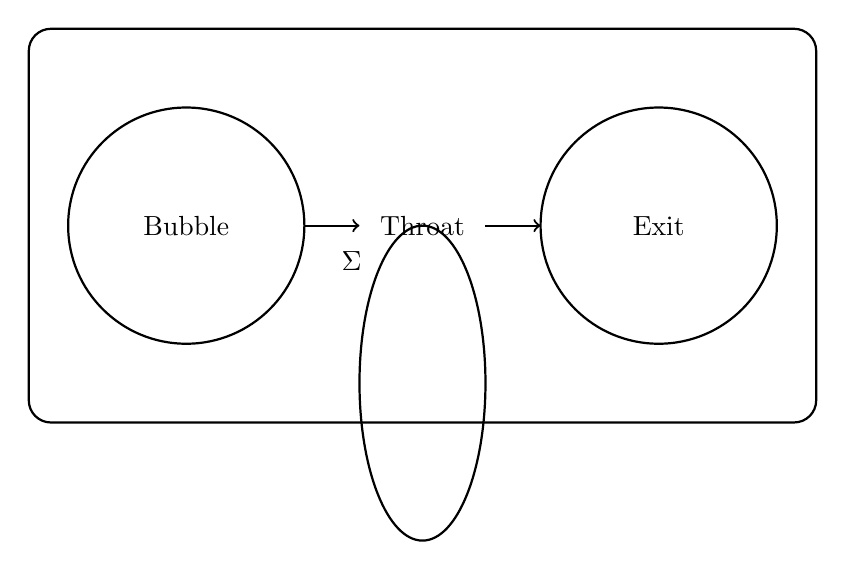
\begin{tikzpicture}[scale=1.0]
  \draw[thick,rounded corners=8pt] (-5, -2.5) rectangle (5, 2.5);
  \draw[thick] (-3,0) circle (1.5); \node at (-3,0) {Bubble};
  \draw[thick] (0,-2) ellipse (0.8 and 2.0); \node at (0,0) {Throat};
  \draw[thick] (3,0) circle (1.5); \node at (3,0) {Exit};
  \draw[->,thick] (-1.5,0) -- (-0.8,0); \draw[->,thick] (0.8,0) -- (1.5,0);
  \node[below] at (-0.9,-0.2) {$\Sigma$};
\end{tikzpicture}
\caption{High-level TikZ sketch of bubble--throat--exit.}
\end{figure}

\section{Figures}
\begin{figure}[h]\centering\includegraphics[width=0.85\linewidth]{figures/bubble_profile.png}\caption{Warp bubble profile (B1--B3).}\end{figure}
\begin{figure}[h]\centering\includegraphics[width=0.85\linewidth]{figures/block_diagram.png}\caption{System block diagram (IBG, NEPA, QIS, JC, EEL).}\end{figure}
\begin{figure}[h]\centering\includegraphics[width=0.85\linewidth]{figures/pulse_shape.png}\caption{Balanced tri-lobe pulse (P1--P4).}\end{figure}
\begin{figure}[h]\centering\includegraphics[width=0.85\linewidth]{figures/solver_outputs/feasible_tau_l_dratio_1.2.png}\caption{Feasible $(\tau,\ell)$, $\Delta/\tau=1.2$.}\end{figure}
\begin{figure}[h]\centering\includegraphics[width=0.85\linewidth]{figures/sweeps/Astar_tau_l_dratio_1.2.png}\caption{$\log_{10}A^\star$ $(\tau,\ell)$, $\Delta/\tau=1.2$.}\end{figure}
\begin{figure}[h]\centering\includegraphics[width=0.85\linewidth]{figures/sweeps/feasible_tau_l_dratio_2.0.png}\caption{Feasible $(\tau,\ell)$, $\Delta/\tau=2.0$.}\end{figure}
\begin{figure}[h]\centering\includegraphics[width=0.85\linewidth]{figures/sweeps/Astar_tau_l_dratio_2.0.png}\caption{$\log_{10}A^\star$ $(\tau,\ell)$, $\Delta/\tau=2.0$.}\end{figure}
\begin{figure}[h]\centering\includegraphics[width=0.85\linewidth]{figures/sweeps/feasible_tau_l_dratio_3.0.png}\caption{Feasible $(\tau,\ell)$, $\Delta/\tau=3.0$.}\end{figure}
\begin{figure}[h]\centering\includegraphics[width=0.85\linewidth]{figures/sweeps/Astar_tau_l_dratio_3.0.png}\caption{$\log_{10}A^\star$ $(\tau,\ell)$, $\Delta/\tau=3.0$.}\end{figure}
\begin{figure}[h]\centering\includegraphics[width=0.85\linewidth]{figures/sweeps/feasible_tau_dratio_l2.0.png}\caption{Feasible $(\tau,\Delta/\tau)$ at $\ell=2.0$.}\end{figure}
\begin{figure}[h]\centering\includegraphics[width=0.85\linewidth]{figures/sweeps/Astar_tau_dratio_l2.0.png}\caption{$\log_{10}A^\star$ $(\tau,\Delta/\tau)$ at $\ell=2.0$.}\end{figure}
\begin{figure}[h]\centering\includegraphics[width=0.85\linewidth]{figures/junction_diagram.png}\caption{Thin-shell matching (I1--I5) and matching (M2).}\end{figure}

\section*{Appendix: Case Study Plots (SI)}
\begin{figure}[h]\centering\includegraphics[width=0.8\linewidth]{figures/case_study/energy_vs_B.png}\caption{Stored magnetic field energy vs $B$ (shell around bubble).}\end{figure}
\begin{figure}[h]\centering\includegraphics[width=0.8\linewidth]{figures/case_study/pressure_vs_B.png}\caption{Magnetic pressure vs $B$.}\end{figure}
\begin{figure}[h]\centering\includegraphics[width=0.8\linewidth]{figures/case_study/energy_vs_R.png}\caption{Stored energy vs bubble radius for $B=20$ T.}\end{figure}

\paragraph{License.} This work is licensed under \textbf{CC-BY 4.0}.

\printbibliography

\end{document}
